\chapter{Tests and Results}
\label{chapter:tests}

This chapter describes the experiments that were performed in order to assess the performance the developed application. The main goals are the following: to obtain an empirical and realistic conclusion about which technology serves better the purpose of this thesis and to assess how the application fares in realistic scenarios.

This chapter will be divided in two different sections: one regarding the comparison between Bluetooth and Wi-Fi Direct in Android devices, and another regarding the tests performed with the developed application, to better understand where it performs better and worse, proving or not if the theoretical choices translate into actual performance gains.

\section{Bluetooth \textit{vs.} Wi-Fi Direct in Android Devices}
\label{sec:btvswifitests}

This section will cover the differences, advantages and disadvantages of both Bluetooth and Wi-Fi Direct. A series of experiments will be conducted and their results analysed, providing a justification on which technology is best suited for this application and applications with a similar architecture and/or purpose. The tests will cover the ranges of communication and discovery times of both technologies.

Since the first implementation of Bluetooth in Android, several releases have been developed. Different Bluetooth versions provide different \gls{QoS}, this may impact the performed tests, as a device running a newer Bluetooth version may provide better results than a device running an older version. For sake of uniformity, all the tested devices will be running Bluetooth version 4.0.

\subsection{Communication Range}
\label{subsec:ranges}

The communication ranges are of extreme importance. They can greatly reduce or increase the number of hops a packet has to pass through, in order to reach the destination. If the range of communication is too short, the number of established connections will increase, which may cause an overload of the network, and the deterioration of communication speed. On the other hand, if the communication range is long, the devices are able to reduce the number of hops, creating less traffic in the network and establishing the least possible number of connections. However, by using a longer communication range the energy consumptions will increase.

Both technologies share some similarities: they depend on the environment of the communication, \textit{i.e.}, the elements that are surrounding the devices and possible obstacles in the way. Four different experiments are conducted, two with line-of-sight and another two without line-of-sight, having walls separating the devices, one for each communication technology. These experiments aim to provide an estimate on the real communication ranges of Bluetooth and Wi-Fi Direct, with and without line-of-sight.

The two non-line-of-sight experiments were conducted in a corridor of Torre Norte, in the vicinities of Instituto Superior Técnico. The Bluetooth line-of-sight experiment was conducted in the same location as the previous experiments. However, the Wi-Fi Direct line-of-sight experiment required a larger environment, so it was conducted in the outside area of Instituto Superior Técnico. It is important to note that, although this experiments were made with as little interference as possible, there are certain elements that are impossible to control, such as wireless communications from other devices and metal objects, such as metal lockers and cars.

Bluetooth establishes four different classes for the devices that may use this technology, depending on the transmitting power. Mobile phones are inserted in class 2 and, for that class, the specified average range of transmission in order to have a reliable connection is \textit{10m}, from \cite{bluetooth}.

Wi-Fi Direct on the other hand offers, theoretically, ranges of communication up to, approximately, \textit{200m} (see \cite{wfdrange}), which represents a much better solution, in terms of network off-loading and general depth.

In order to verify these claims from both technologies, two mobile devices were taken to an open space, although with some limitations as described above, and several discovery procedures were made, until the devices stopped being discovered by one another. Both tests were made with a direct line-of-sight between devices.

Bluetooth was able to create a connection between devices from a distance up to \textit{42m} apart (see Figure \ref{fig:btMaxVisib} for the overall scheme of this experiment). This value is higher than what was expected judging by the theoretical value of \textit{10m}, although the quality of the connection was not verified -- see Section \ref{sec:btvswifi} to see how the distance affects the data rates. Using Wi-Fi Direct, the devices were able to communicate from a maximum distance of \textit{77m} (see Figure \ref{fig:wfdMaxVisib} for the overall scheme of this experiment, which is considerably lower than the theoretical value of \textit{200m}).

\begin{figure}[ht]
   \noindent\makebox[\textwidth]
    {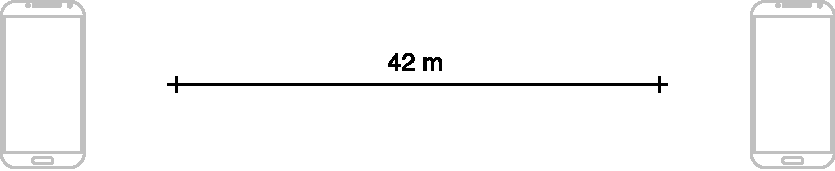
\includegraphics[width=0.8\textwidth]{images/bt_max_visib.pdf}}
	\caption{\label{fig:btMaxVisib} Max range of Bluetooth communication with line-of-sight between devices.}
\end{figure}

\begin{figure}[ht]
   \noindent\makebox[\textwidth]
    {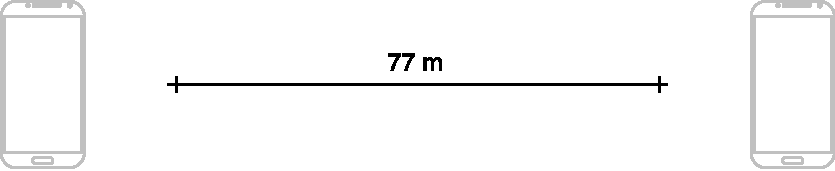
\includegraphics[width=0.8\textwidth]{images/wfd_max_visib.pdf}}
	\caption{\label{fig:wfdMaxVisib} Max range of Wi-Fi Direct communication with line-of-sight between devices.}
\end{figure}

The other experiment concerns non-line-of-sight communication. It is expected that the walls standing between devices will affect significantly the communication ranges, since walls block possible signal reflections. The first test was made using Bluetooth technology where a wall was blocking the line-of-sight between devices -- see Figure \ref{fig:btMaxInv}. The second test was made using Wi-Fi Direct, and, in order to maintain the same scenario as the previous experiment, it was located in the same place as the first -- see Figure \ref{fig:wfdMaxInv}. However, due to the scenario configuration, it was impossible to recreate the experiment with only one wall, so two walls are now dividing the devices. Since the walls introduce a loss in the signal power, the more walls stand between devices, the bigger the losses will be.

\begin{figure}[ht]
   \noindent\makebox[\textwidth]
    {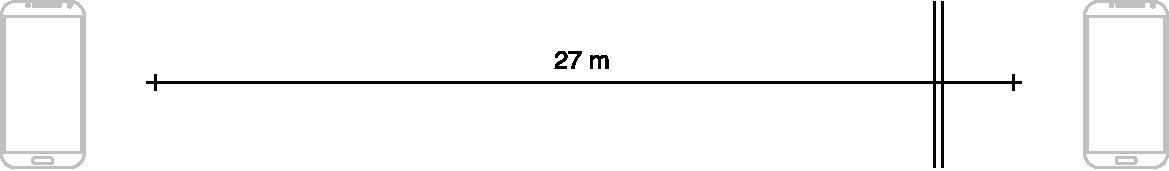
\includegraphics[width=0.8\textwidth]{images/bt_max_inv.pdf}}
	\caption{\label{fig:btMaxInv} Max range of Bluetooth communication without line-of-sight between devices.}
\end{figure}

\begin{figure}[ht]
   \noindent\makebox[\textwidth]
    {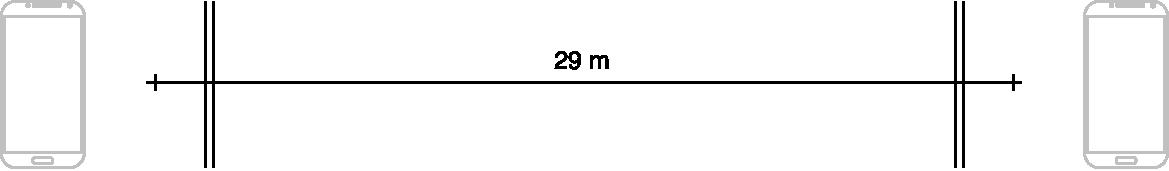
\includegraphics[width=0.8\textwidth]{images/wfd_max_inv.pdf}}
	\caption{\label{fig:wfdMaxInv} Max range of Wi-Fi Direct communication without line-of-sight between devices.}
\end{figure}

As expected, the wall created a significant decrease on the maximum range of communication. The devices were able to communicate via Bluetooth from a distance of \textit{27m}, closer to the theoretical \textit{10m}.

Wi-Fi Direct was also able to communicate from a shorter maximum distance, measuring \textit{29m} with the signal passing through both walls. From a shorter distance, it was verified that this technology could communicate with only one wall in the way, meaning it also surpasses Bluetooth when an obstacle blocks the line-of-sight.

After these experiments, it is possible to conclude that Wi-Fi Direct is more advantageous, since it provides better coverage than Bluetooth to similar areas. Also, there is no evidence that Wi-Fi Direct suffers more losses from obstacles. This was already to expect, both from the theoretical values and from the transmission powers\footnote{Transmission powers impact directly the range of transmission, since they affect the signal strength, a crucial characteristic for receivers to better capture the transmissions. A higher transmit power, usually, creates a stronger signal strength leading to the signal being capture over longer distances, as referred in \cite{txpower}, for instance.}, since Bluetooth is characterized by lower transmit powers, when compared with Wi-Fi.

\subsection{Discovery Times}
\label{subsec:normaldisc}

The discovery time is a critical factor for this work. The discovery process is one of the biggest time consumers during an application run. Thus, minimizing it, is a great advantage for the overall performance of the application.

For the purpose of testing the Bluetooth and Wi-Fi Direct discovery times, three mobile devices were used: Samsung Grand Neo, running Android version 4.2.2; Motorola Moto G2, running Android version 7.1; Huawei P8 Lite, running Android version 6.0, providing an heterogeneous sample space.

Every device is running Bluetooth version 4.0, as previously stated. This Bluetooth version theoretically provides a discovery time of \textit{10.24s}, as mentioned in \cite{bluetoothspec}, \cite{btdisc1} and \cite{btdisc2}. To confirm this hypothesis, discovery times values from the three devices were measured. Each device was submitted to multiple discoveries with a different number of discovered peers, ranging from 0 to 3.

Figure \ref{fig:normaldisc} shows the measured Bluetooth discovery times from the three tested devices. It is important to note that these results were measured with a chronometer, having a maximum precision of \textit{0.5s}.

Samsung Grand Neo (in blue) is constant throughout the measuring, having a Bluetooth discovery time of \textit{13s}. Motorola Moto G2 (in green) shows some variance in the various measurements. The Bluetooth discovery time ranges between \textit{13s} and \textit{14s}, having an average of \textit{13.85s}. Huawei P8 Lite (in purple) shows the biggest deviation throughout the sample space. Its Bluetooth discovery time ranges between \textit{16.5s} and \textit{15s}, having an average of \textit{15.976s}.

\begin{figure}[ht]
	\noindent\makebox[\textwidth]
	{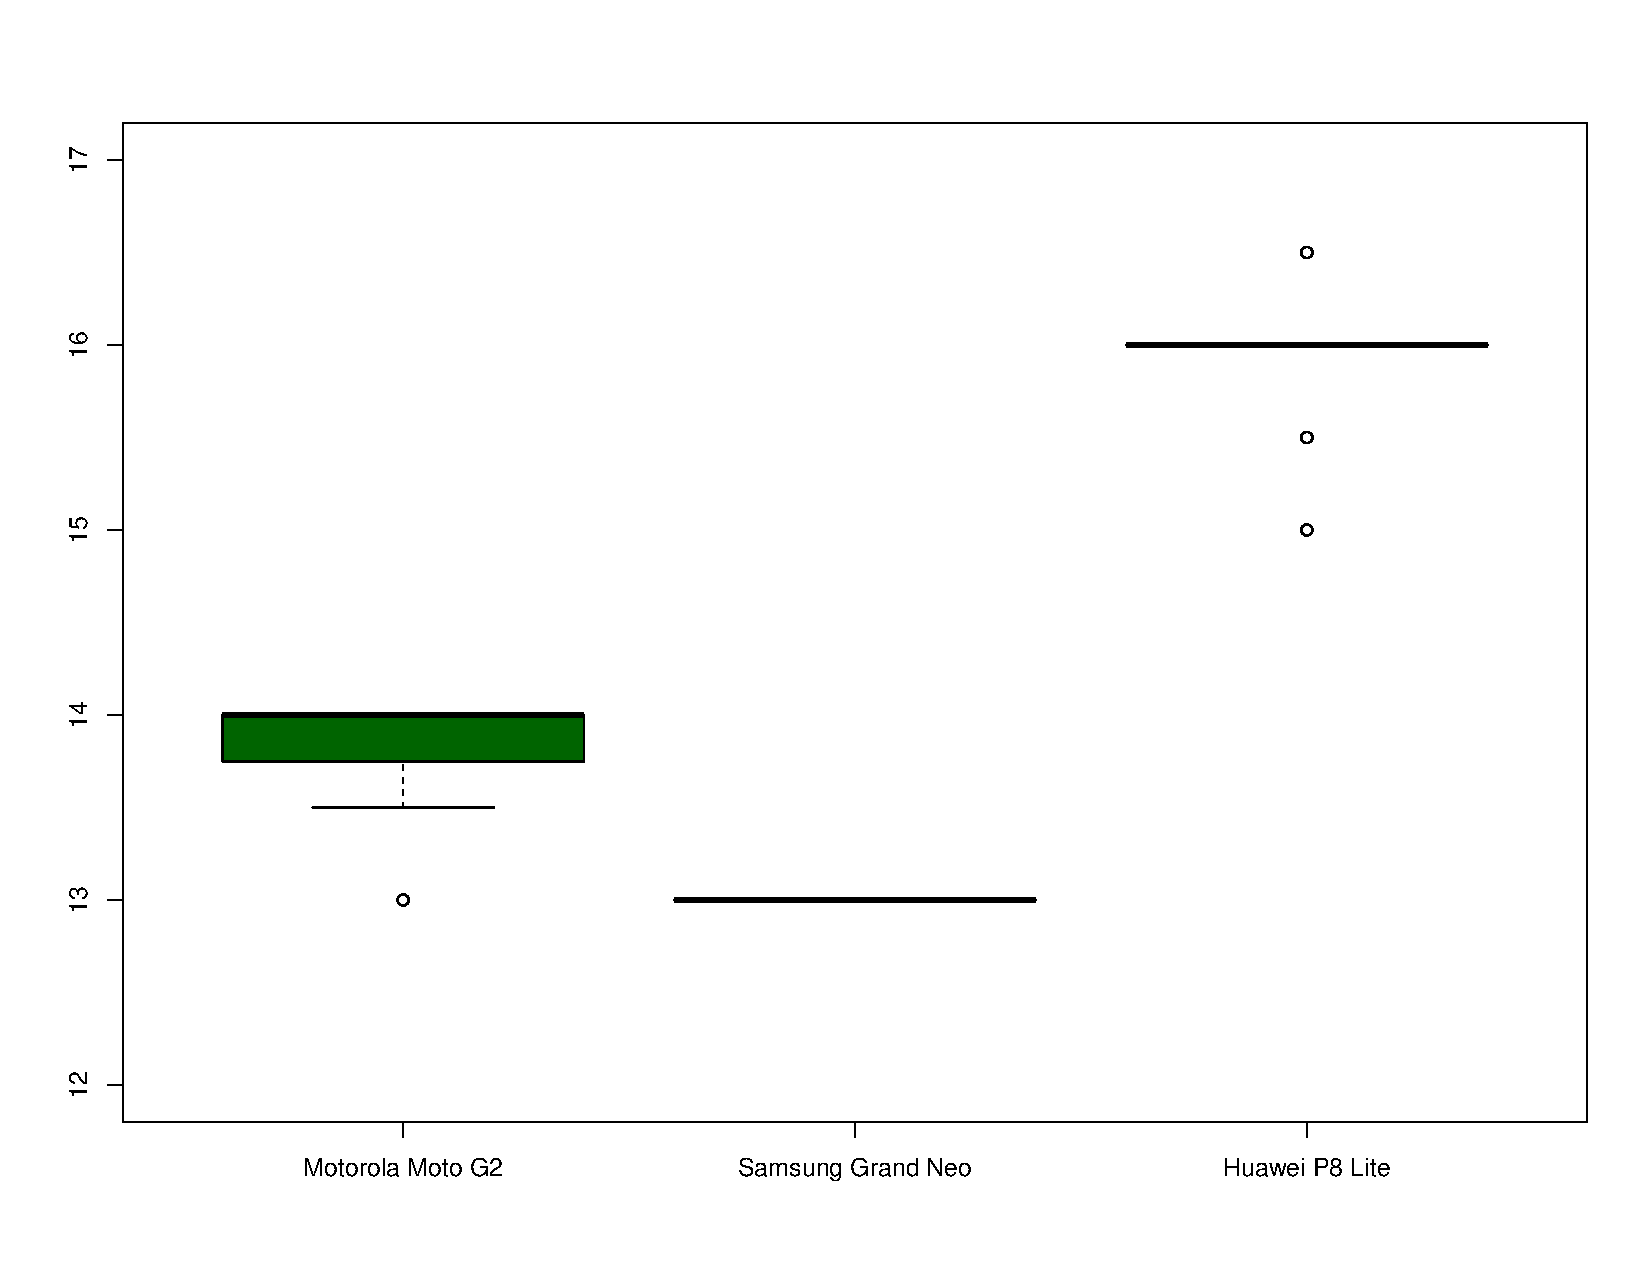
\includegraphics[width=1.2\textwidth]{images/boxplot_normal_disc.pdf}}
	\caption{\label{fig:normaldisc} Boxplot of the measured Bluetooth discovery times from the three devices.}
\end{figure}

None of the three devices approached the theoretical Bluetooth discovery time value of \textit{10.24s}. The difference is quite significant in a delay-sensitive application, such as the developed one.

Each device showed a different average Bluetooth discovery time. This difference in the discovery times can be due to the different hardware used in the devices, since each device is produced by a different manufacturer.

Wi-Fi Direct, on the other hand, does not provide a discovery time limit. This technology is constantly scanning for peer devices, until the stops the ongoing search -- see \cite{wfddisc}. This is also a cause for Wi-Fi Direct's higher energy consumption, since this process is running in background when the technology is being used.

\section{Testing the Developed Application}

This section describes a sequence of tests aiming to provide an overview of the developed application's performance. The main processes of the developed applications will be tested: the discovery, advertisement and web page exchange process.

\subsection{Discovery Times}
\label{subsec:appdisc}

To obtain a meaningful analysis the devices used are the same as the ones in Subsection \ref{subsec:normaldisc}. It is expected that the measured discovery time values don't differ greatly from the ones previously obtained.

In this experiment the number of discovered peer devices also ranges from 0 to 2. However, to retrieve the Bluetooth discovery times from the developed application the Android debugger was used, providing a precision of \textit{0.5ms}.

In Figure \ref{fig:appdisc}, the times measured during the developed application's discovery procedure are shown. Analysing the boxplot it is possible to see that (1) Samsung Grand Neo (in blue) shows the best Bluetooth discovery times, being almost constant throughout the sample space -- it provides an average discovery time of \textit{12.826s}; (2) Motorola Moto G2's (in green) discovery times were similar to Samsung Grand Neo's discovery times, except for punctual samples, where the times are slightly higher -- it provides an average discovery time of \textit{12.991s}; (3) Huawei P8 Lite (in purple) provides the most irregular measures, similarly to what happened in Subsection \ref{subsec:normaldisc} -- its measured times range from \textit{15s} to \textit{18s}, having an average of \textit{16.755s}.

\begin{figure}[ht]
	\noindent\makebox[\textwidth]
	{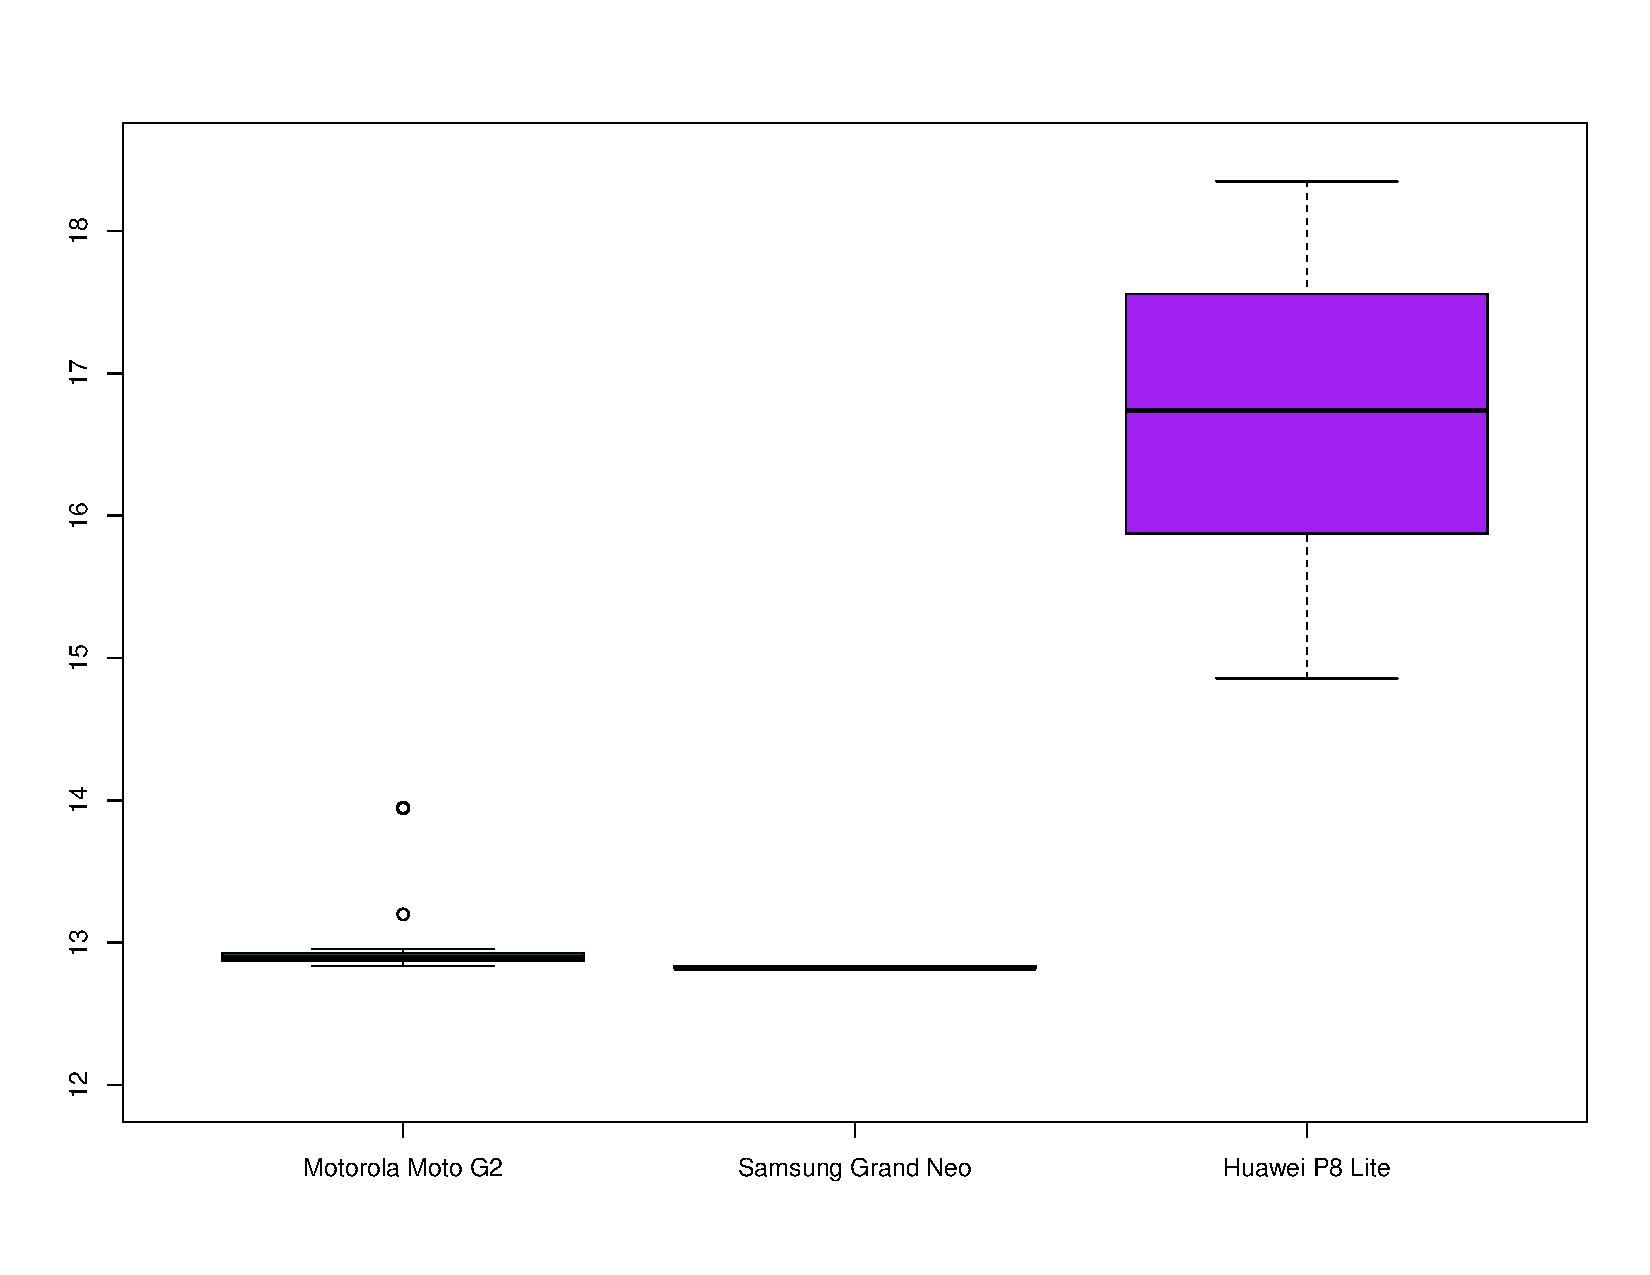
\includegraphics[width=1.2\textwidth]{images/boxplot_app_disc.pdf}}
	\caption{\label{fig:appdisc} Boxplot of the Bluetooth discovery times measured while using the developed application from the three devices.}
\end{figure}

As expected, the measured application discovery times were very similar to the ones obtained during a native discovery time. All the devices maintained the same properties in the two scenarios: Samsung Grand Neo was mostly constant in both tests, providing the lowest discovery times; Motorola Moto G2 provided the second best discovery times, showing less deviation from the average in the current test than during the test performed in \ref{subsec:normaldisc}; Huawei P8 Lite showed the worst discovery times, however its average discovery time was similar in both tests. It also showed the most deviation from the average in both tests, having a larger amplitude of results in the current test, as mentioned before.

Once again, it is possible to see that all three devices failed to meet the theoretical value of \textit{10.24s}, having shown discovery time averages of the theoretical time plus \textit{2s} to \textit{4s}.

\subsection{Advertisement Times}

In this subsection, the advertisement times are measured and analysed. There are two sets of tests: one where devices advertise to one peer and another one where devices advertise to two peers. These two sets of tests aim to provide a better understanding on how much time the advertisement process occupies during an application run.

The devices used to test the advertisement process duration are the same used in the previous test: Motorola Moto G2, Samsung Grand Neo and Huawei P8 Lite. Since the application needs to establish one connection per peer device found, it is expected that the advertisement times to one peer will be slightly lower than the advertisement times to two peers, although the difference should not impact the overall application runtime.

In Figure \ref{fig:adv1} it is possible to see a boxplot of the advertisement times of the three devices. Analysing the boxplot, it is possible to see that (1) Motorola Moto G2 has the lowest average advertisement time, as well as the lowest standard deviation from the three devices -- it provides, approximately, a maximum of \textit{2s} and a minimum of \textit{0.75s}, having an average advertisement time of \textit{1.333s}; (2) Unlike the tests in Subsection \ref{subsec:appdisc}, Samsung Grand Neo has the highest standard deviation, covering the highest and lowest advertisement time values from the three devices -- it provides, approximately, a maximum advertisement time of \textit{3.5s} and a minimum of \textit{0.35s}, having an average advertisement time of \textit{1.514s}; (3) Huawei P8 Lite has most of its values in the interval between \textit{1.75s} and \textit{1s} -- it provides, approximately, a maximum of \textit{2s} and a minimum advertisement time of \textit{0.75s}, having an average advertisement time of \textit{1.388s}.

\begin{figure}[ht]
	\noindent\makebox[\textwidth]
	{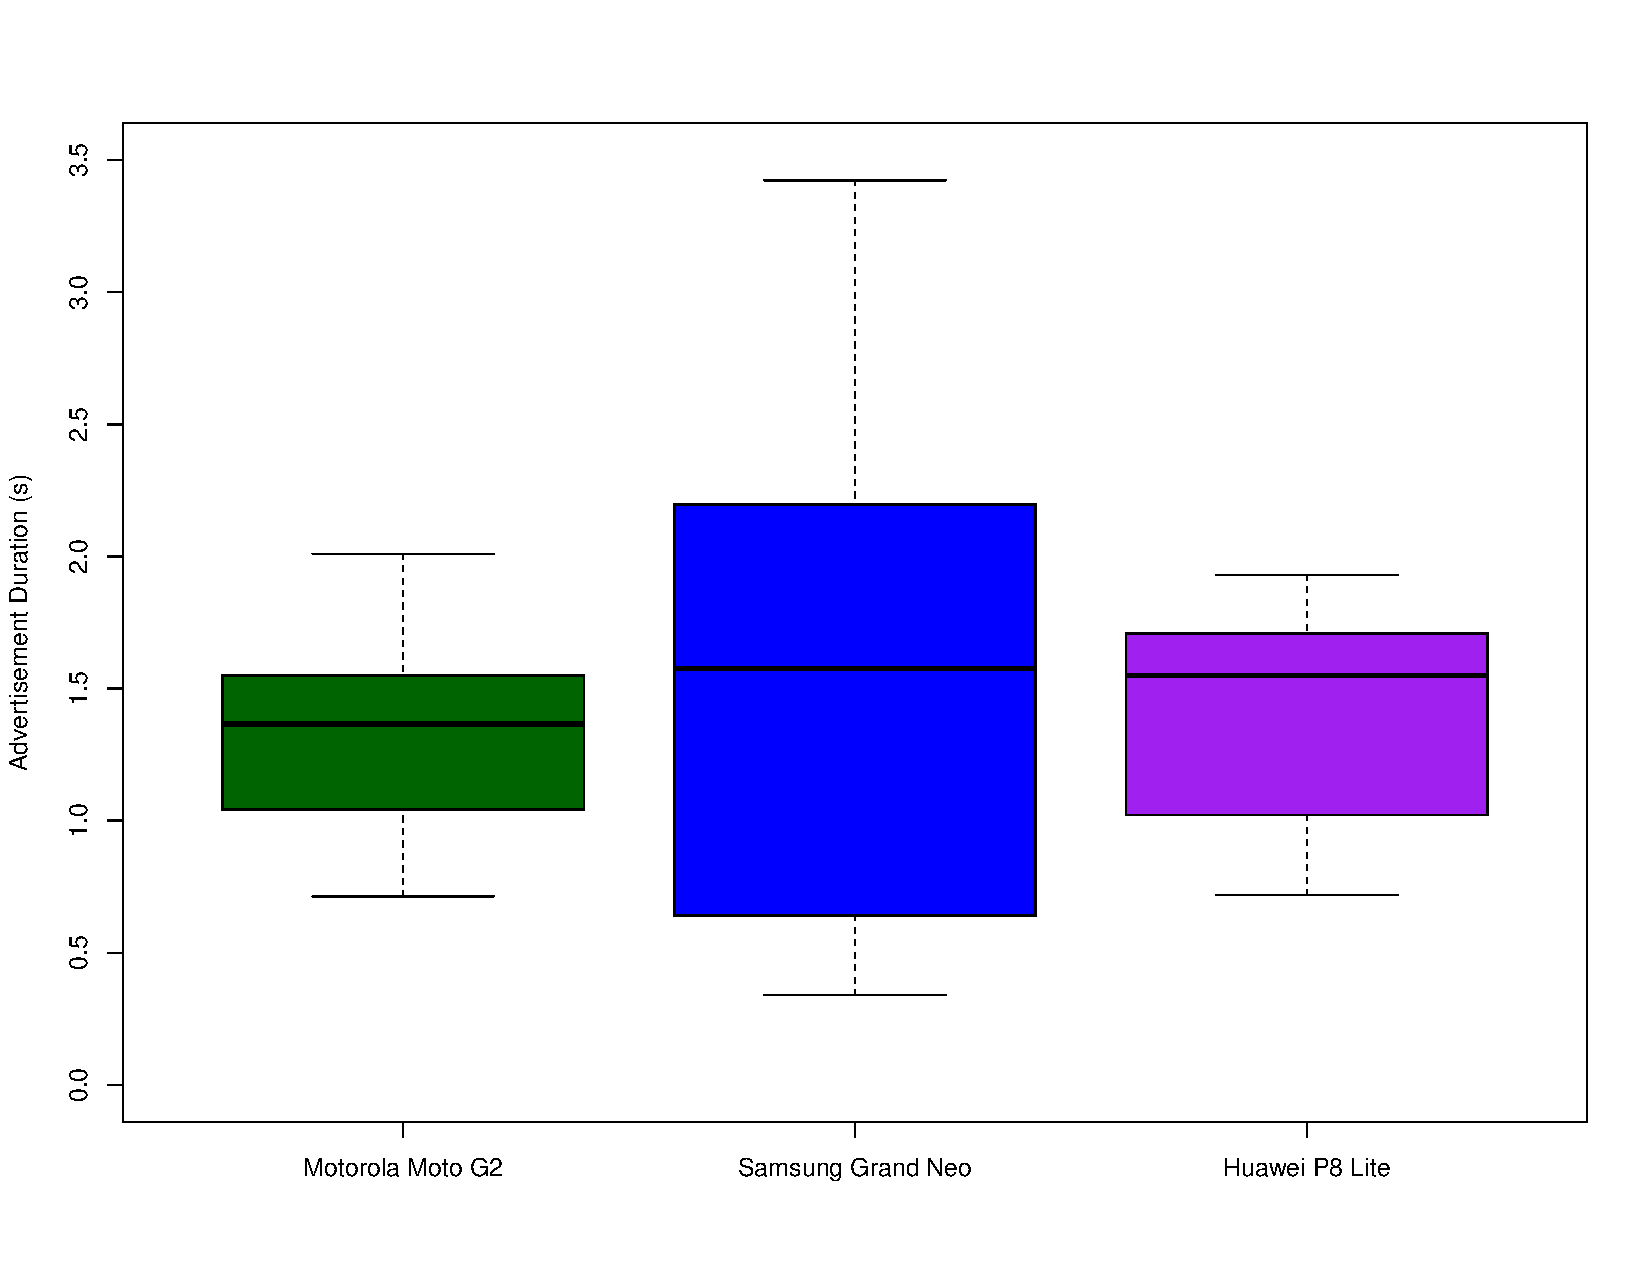
\includegraphics[width=1.2\textwidth]{images/boxplot_adv_1.pdf}}
	\caption{\label{fig:adv1} Boxplot of the advertisement times towards one peer measured while using the developed application from the three devices.}
\end{figure}

All three tested devices provide a similar average advertisement time. In the next test, these devices will advertise to two distinct peers. In Figure \ref{fig:adv2}, it is possible to see a boxplot of three advertisement durations of the three tested devices. It is also visible that the disparity between durations is significantly higher than in the previous experiment, due to the supplementary complexity of advertising to more than one peer and establishing the individual connections.

In the boxplot of Figure \ref{fig:adv2}, it can be seen that (1) Motorola Moto G2's advertisement times range from, approximately, \textit{1.8s} to \textit{5.2s}, having an average advertisement time of \textit{3.066s} -- in comparison with the previous test, the amplitude of advertisement durations is now of around \textit{3.4s}, compared to the previous \textit{1.25s}; (2) Samsung Grand Neo, similarly to the previous test, shows the biggest disparity of results, ranging from \textit{1.7s} to \textit{7s}, approximately, also having a higher amplitude of \textit{6.3s}, than the previously measured \textit{3.15s} -- it provides an average advertisement time towards two peers of \textit{3.449s}; (3) Huawei P8 Lite shows the smallest standard deviation, having measures ranging from \textit{2.2s} to \textit{4.1s} -- this device provides an average advertisement time towards two peers of \textit{3.414s}.

\begin{figure}[ht]
	\noindent\makebox[\textwidth]
	{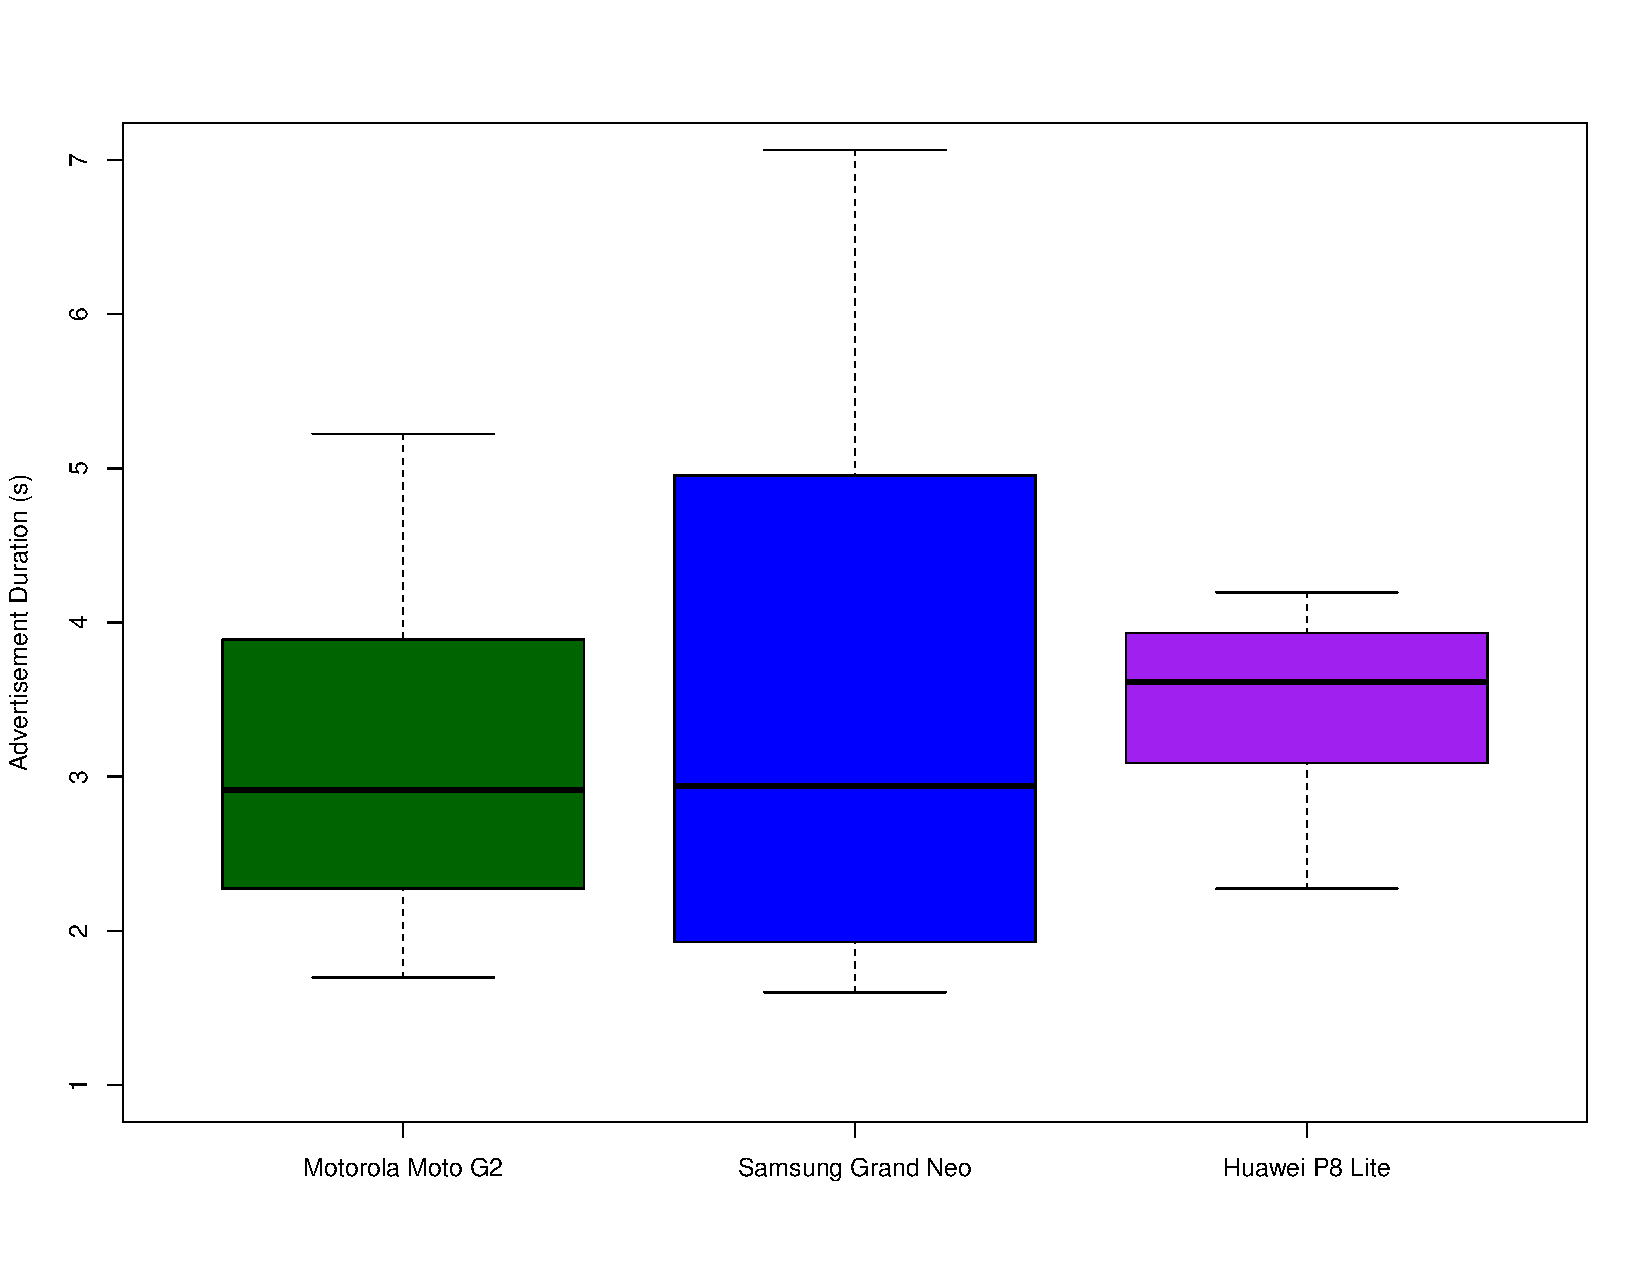
\includegraphics[width=1.2\textwidth]{images/boxplot_adv_2.pdf}}
	\caption{\label{fig:adv2} Boxplot of the advertisement times towards two peers measured while using the developed application from the three devices.}
\end{figure}

Reflecting on the results of these two experiments, it is plausible to say that, the advertisement times are independent of the device where the application is running. The advertisement times between experiments were slightly different, as was expected. Since individual connections must be established between advertiser and its peers, the first experiment sets the base advertisement time, as it reflects a one-to-one advertisement. The second experiment reflects a one-to-two advertisement and, the measured average times are double the one-to-one advertisement times, approximately.

The results of the different experiments suggest that the advertisement time is given by, approximately, the base advertisement time times the number of peers being advertised to. Although this is not confirmed, due to lack of testing equipment.

\subsection{Web Page Exchange Throughput}

In this subsection, the web page exchange data rates will be measured and analysed. Moreover, to better understand where the developed framework and application are wasting more time, an analysis of the time spent in each process will be shown.

To measure the throughput and percentage of time spent by each process, four scenarios were considered: 

\begin{itemize}
	\item The first scenario used two devices, one acting as client and another one acting as server, similar to what was shown in Figure \ref{fig:adveg1}. A web page with \textit{1.9KB} was transferred (\url{https://www.example.com}).
	
	\item The second scenario maintained the same network topology. However the transferred web page was larger, sizing \textit{105.5KB} (\url{https://www.google.com}).
	
	\item The third scenario used three devices, one acting as client, one as relay node and one as server, similar to the topology shown in Figure \ref{fig:example1.0}. The transferred web page was the same as in the first scenario.
	
	\item The fourth scenario used the same topology as before. However, the transferred web page corresponded to the one used in the second scenario, with \textit{105.5KB}.
\end{itemize}

Before analysing the plots, it is important to understand what processes are present in the web page exchange, described in Subsection \ref{subsec:exch}, and how was the throughput measured. Since there are two different network topologies, there will be different processes to be analysed, depending on the experiment.

In the first two experiments, two devices are used, meaning (1) one request is issued from the client to the server (\textit{Request \#1}); (2) the web page is downloaded (\textit{Download Web Page}); (3) the response is sent from the server to the client (\textit{Response \#1}); (4) the web page is transferred from the server to the client (\textit{Web Page Transfer \#1}).

In the third and fourth experiments, three devices are used, meaning (1) a request from the client to the relay node is sent (\textit{Request \#1}); (2) the request is forwarded from the relay to the server node (\textit{Request \#2}); (3) the web page is downloaded (\textit{Download Web Page}); (4) a response is sent from the server to the relay node (\textit{Response \#1}); (5) the web page is transferred from the server to the relay node (\textit{Web Page Transfer \#1}); (6) the reponse is forwarded from the relay node to the client (\textit{Response \#2}); (7) the web page is transferred from the relay node to its final destination (\textit{Web Page Transfer \#2}).

To measure the throughput in the first and second scenarios, the number of transferred bits are divided by the number of seconds that the application took to accomplish processes \textit{Response \#1} and \textit{Web Page Transfer \#1}.

In the third and fourth scenarios, the throughput was measured by dividing the transferred bits by the number of seconds that the application took to conclude the processes of \textit{Response \#1}, \textit{Web Page Transfer \#1}, \textit{Response \#2} and \textit{Web Page Transfer \#2}.

The \textit{Download Web Page} and previous processes were not taken into account when measuring the throughput, as their durations are dependent on the server node's Internet connection quality.

In Figure \ref{fig:boxplotthroughput}, the measured throughputs in the previously described scenarios are shown. In both the first and third scenarios, the average throughput is approximately \textit{0.3Mbps}. Also, if compared to the other two scenarios, it is possible to see that the standard deviations are greater. This is mainly due to the small duration of the web page exchange, making the measuring harder and less precise. The second and fourth scenarios provide similar results, with an average throughput of roughly \textit{0.75Mbps} and lower standard deviation.

\begin{figure}[ht]
	\noindent\makebox[\textwidth]
	{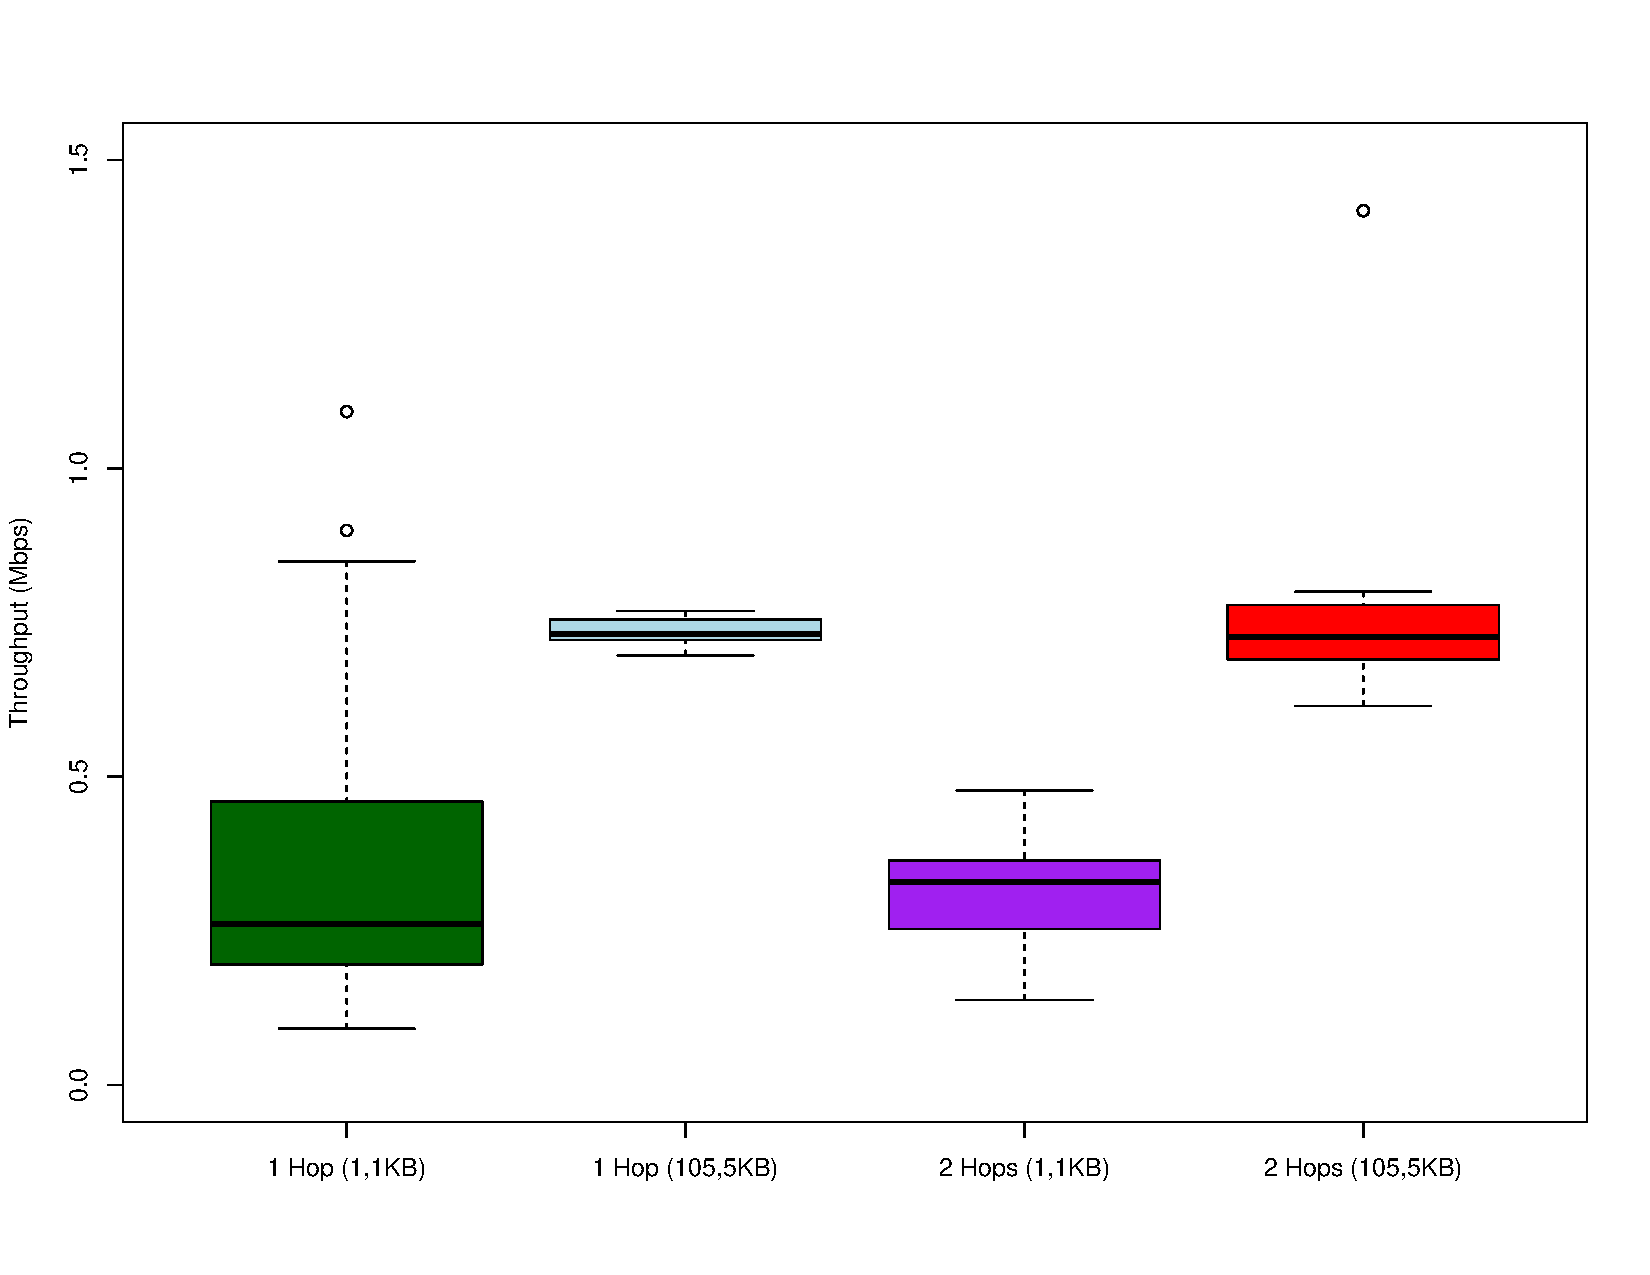
\includegraphics[width=1.2\textwidth]{images/boxplot_data_rates.pdf}}
	\caption{\label{fig:boxplotthroughput} Boxplot of the measured throughput in the different experiment scenarios.}
\end{figure}

The results seen in Figure \ref{fig:boxplotthroughput} are to be expected since, when exchanging smaller web pages, the connection and application specific computation delays, such as the queries to the Response Table to retrieve the next hop and the analysis of the received data, have a more significant impact in the overall delay than when exchanging larger web pages. Hence, the lower average throughput measured in the first and third scenarios and higher average throughput in the remaining scenarios.

If compared to the results shown in Subsection \ref{sec:btvswifi}, the measured throughputs are lower than the Bluetooth indoor line-of-sight throughput measured at a distance of \textit{0m}. In this experiment, the maximum average throughput obtained was of approximately \textit{0.75Mbps}, a value lower than the obtained value of \textit{2Mbps} (see Figure \ref{fig:btin}). This difference is again justified with the delays introduced by the connections and application specific computations during the exchange of web pages.

To measure the percentage of time spent by each of the processes described above, the duration of that process was divided by the total duration of the web page exchange, since the initial request is sent until the final web page is received by the destination.

In Figure \ref{fig:perctime}, a barplot is presented, showing the different percentages of time each process took, in each scenario. Starting from left to right (first to last scenario), it is possible to see that:

\begin{enumerate}
	\item In the first scenario the majority of time was spent downloading the web page, representing over \textit{70\%} of the total duration. The remaining processes' durations sum up to less than \textit{10\%} of the total duration.
	
	\item The second scenario shows that two processes occupy most of the total duration, \textit{Download Web Page} and \textit{Web Page Transfer \#1}. Combined, they sum more than \textit{90\%} of the total duration, representing roughly \textit{50\%} and \textit{40\%} of the web page exchange's duration, respectively. The remaining processes are almost insignificant in the overall duration of the web page exchange.
	
	\item The third scenario shows a similar process distribution to the first scenario, with the \textit{Download Web Page} process occupying significantly more than the rest, around \textit{30\%}. It is also seen that, despite more processes being measured, the total duration of the processes reaches less than \textit{35\%} of the total duration.
	
	\item In the fourth scenario, the most time costly processes are \textit{Download Web Page}, \textit{Web Page Transfer \#1} and \textit{Web Page Transfer \#2}. Together, they represent close to \textit{70\%} of the total duration. The remaining processes are insignificant, summing up to little more than \textit{1\%} of the total duration.
\end{enumerate}

Figure \ref{fig:perctime} also shows that, in the first and third scenarios, where the web page is smaller, the majority of time is occupied downloading it, as the transfer between devices of such a small number of bytes is almost immediate. It is also possible to see that, in this scenarios, the percentage of time occupied by the measured processes is less than in the scenarios with the same topology but where a larger web page is transferred, due to the connection establishment and application specific computation delays occupying a larger portion of the web page exchange duration. In the second and fourth scenarios, these delays occupy a smaller portion of time, since the download and transfers of the web page are longer.

\begin{figure}[ht]
	\noindent\makebox[\textwidth]
	{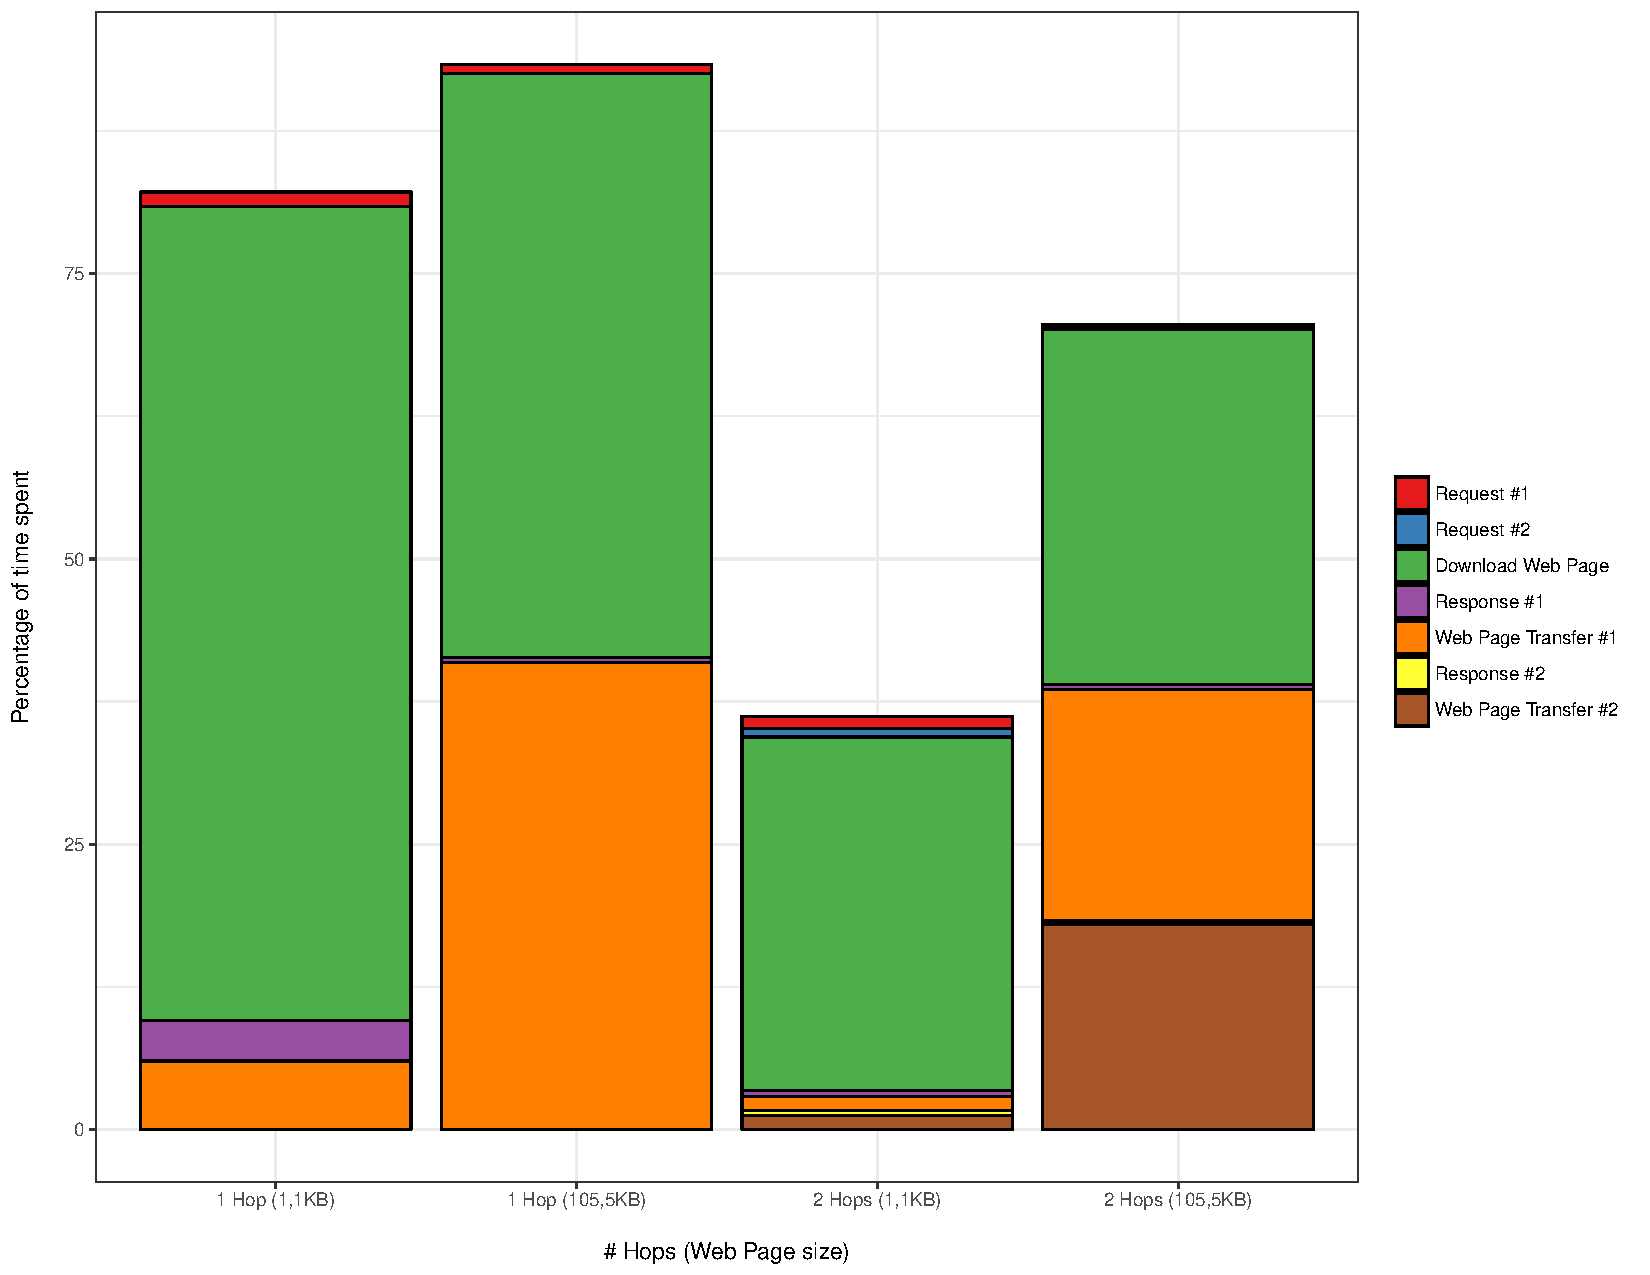
\includegraphics[width=1.2\textwidth]{images/barplot_ftt_perc.pdf}}
	\caption{\label{fig:perctime} Barplot of the percentage of occupied by the various processes in the different experiment scenarios.}
\end{figure}

As expected, when the web page size is larger, so is the portion of time occupied by its transfer. The request and response sending processes are mostly insignificant, introducing little delay in the web page exchange process. Also as expected, in the third and fourth scenarios, the \textit{Web Page Transfer \#1} and \textit{Web Page Transfer \#2} processes occupy a similar percentage of the web page exchange duration, as the same number of bytes is being sent over a similar link.

As mentioned before, these results are influenced by the server node's Internet connection quality, impacting the duration the \textit{Download Web Page} process, especially when dealing with larger web pages.




